%\documentstyle[epsf,twocolumn]{jarticle}       %LaTeX2e仕様
\documentclass[twocolumn]{jarticle}     %pLaTeX2e仕様(platex.exeの場合)
% \documentclass[onecolumn]{ujarticle}   %pLaTeX2e仕様(uplatex.exeの場合)
%%%%%%%%%%%%%%%%%%%%%%%%%%%%%%%%%%%%%%%%%%%%%%%%%%%%%%%%%%%%%%
%%
%%  基本バージョン
%%
%%%%%%%%%%%%%%%%%%%%%%%%%%%%%%%%%%%%%%%%%%%%%%%%%%%%%%%%%%%%%%%%
\setlength{\topmargin}{-45pt}
%\setlength{\oddsidemargin}{0cm}
\setlength{\oddsidemargin}{-7.5mm}
%\setlength{\evensidemargin}{0cm}
\setlength{\textheight}{24.1cm}
%setlength{\textheight}{25cm}
\setlength{\textwidth}{17.4cm}
%\setlength{\textwidth}{172mm}
\setlength{\columnsep}{11mm}

%\kanjiskip=.07zw plus.5pt minus.5pt


% 【節が変わるごとに (1.1)(1.2) … (2.1)(2.2) と数式番号をつけるとき】
%\makeatletter
%\renewcommand{\theequation}{%
%\thesection.\arabic{equation}} %\@addtoreset{equation}{section}
%\makeatother

%\renewcommand{\arraystretch}{0.95} 行間の設定
%%%%%%%%%%%%%%%%%%%%%%%%%%%%%%%%%%%%%%%%%%%%%%%%%%%%%%%%
%\usepackage{graphicx}   %pLaTeX2e仕様(\documentstyle ->\documentclass)
\usepackage[dvipdfmx]{graphicx}
\usepackage{subcaption}
\usepackage{multirow}
\usepackage{amsmath}
\usepackage{url}
\usepackage{ulem}
\usepackage{algorithm}
\usepackage{algorithmic}
\usepackage{listings} %,jlisting} %日本語のコメントアウトをする場合jlistingが必要
%ここからソースコードの表示に関する設定
\lstset{
  basicstyle={\ttfamily},
  identifierstyle={\small},
  commentstyle={\smallitshape},
  keywordstyle={\small\bfseries},
  ndkeywordstyle={\small},
  stringstyle={\small\ttfamily},
  frame={tb},
  breaklines=true,
  columns=[l]{fullflexible},
  numbers=left,
  xrightmargin=0zw,
  xleftmargin=3zw,
  numberstyle={\scriptsize},
  stepnumber=1,
  numbersep=1zw,
  lineskip=-0.5ex
}
%%%%%%%%%%%%%%%%%%%%%%%%%%%%%%%%%%%%%%%%%%%%%%%%%%%%%%%%
\begin{document}

	%bibtex用の設定
	%\bibliographystyle{ujarticle}

	\twocolumn[
		\noindent
		\hspace{1em}
		2020 年 10 月 9 日
		ゼミ資料
		\hfill
		B4 杉山 竜弥
		\vspace{2mm}

		\hrule
		\begin{center}
			{\Large \bf 進捗報告}
		\end{center}
		\hrule
		\vspace{9mm}
	]

	% ‚ここから 文章 Start!
% \section{今週やったこと}
% \begin{itemize}
% 	\item グラフ距離の計算
% \end{itemize}

\section{問題}
前回同様.

初期条件として探索をベースラインのVGG19に相当する$\alpha$から始めた.

\section{実験}

\begin{table}[tb]
  \begin{center}
    \caption{実験の設定}
    \begin{tabular}{|c|c|} \hline
      model & VGG19 \\ \hline
      Optim($w$) & SGD(lr=0.01, momentum=0.9) \\ \hline
      Optim($\alpha$) & Adam(lr=0.005, $\beta$=(0.5, 0.999)) \\ \hline
      Loss & Cross Entropy Loss \\ \hline
      dataset & cifar10 \\ \hline
      batch size & 64 \\ \hline
    \end{tabular}
    \label{tab:setting}
  \end{center}
\end{table}

表\ref{tab:setting}に探索時の実験設定を示した.

評価段階では, SGDの学習率を, 指数スケジューラ($\gamma = 0.9261 : \gamma^{30} = 0.1$)で減衰させた.

\begin{description}
  \item[(a) descending] $\alpha_j$の上位から順に, $\rm{round}(\hat{\beta_j})$本のショートカットを選んだグラフ,
  \item[(b) threshold] $\hat{\alpha}_{ij} >= 0.5$となるショートカットを選んだグラフ,
  \item[(c) baseline] ショートカットをすべて破棄したグラフ,
\end{description}
の3つで性能を評価した.

\subsection{結果}

\begin{table*}[tb]
  \begin{center}
    \caption{各条件の比較}
    \begin{tabular}{|c||c|c|c|c|c|c|c|} \hline
       & テスト精度  & 学習時間 & 計算時間 & パラメータ数 & \multicolumn{3}{c|}{データサイズ} \\
       & (\%)  & (epoch) & (GPU-min) & & train & valid & test \\ \hline \hline
      探索 & 87.24 & 50 & 120 & 26.30M & 25000 & 25000 & 5000 \\ \hline
      (a) descending & 92.14 & 100 & 120 & 20.85M & 50000 & 0 & 10000 \\ \hline
      (b) threshold & 91.83 & 100 & 120 & 20.27M & 50000 & 0 & 10000 \\ \hline
      (c) baseline & 91.79 & 100 & 120 & 20.04M & 50000 & 0 & 10000 \\ \hline
    \end{tabular}
    \label{tab:acc}
  \end{center}
\end{table*}

\begin{figure}[tb]
	\begin{center}
		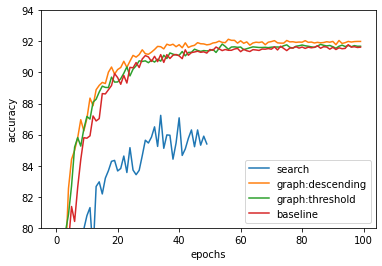
\includegraphics[clip,width=75mm]{acc.png}
		\caption{学習中のテスト精度}
		\label{fig:acc}
	\end{center}
\end{figure}

\begin{figure}[tb]
	\begin{center}
		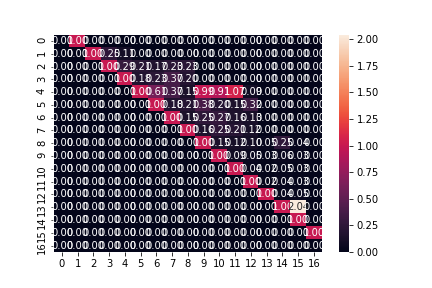
\includegraphics[clip,width=85mm]{alpha_50.png}
		\caption{探索後の隣接行列の重み$\hat{\alpha}$}
		\label{fig:alpha}
	\end{center}
\end{figure}

図\ref{fig:acc}にテスト精度を, 表\ref{tab:acc}に結果を示した.

\begin{figure*}[tb]
  \begin{tabular}{ccc}
    %---- 最初の図 ---------------------------
    \begin{minipage}[t]{0.3\hsize}
      \centering
      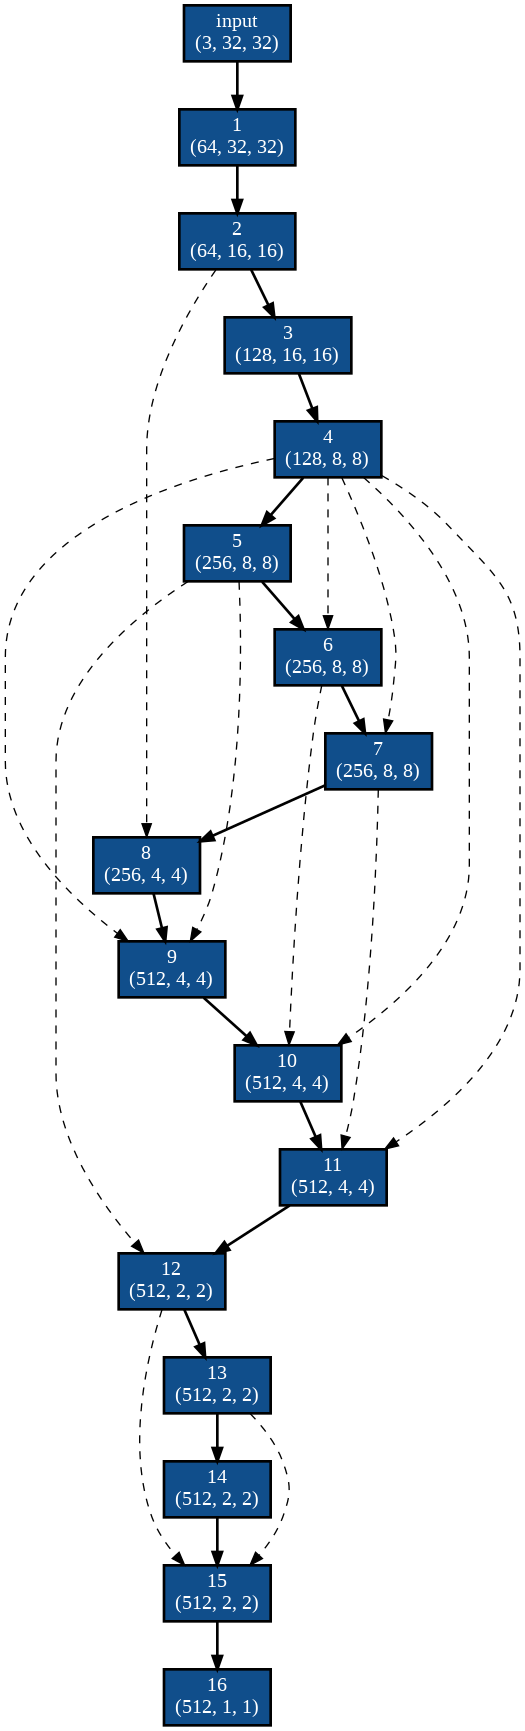
\includegraphics[clip,scale=0.25]{max.png}
      \caption{グラフ(a)}
      \label{fig:max}
    \end{minipage} &
    %---- 2番目の図 --------------------------
    \begin{minipage}[t]{0.3\hsize}
      \centering
      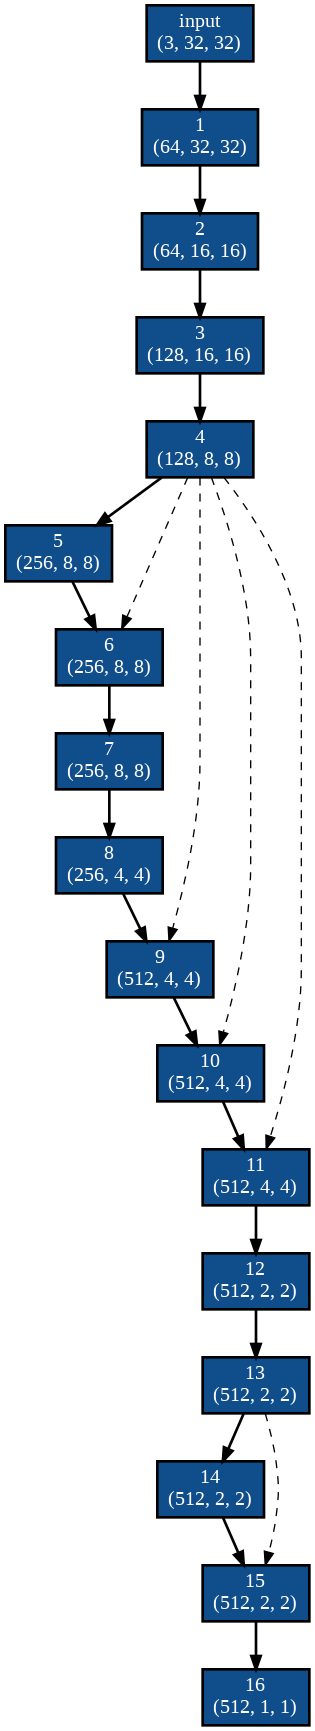
\includegraphics[clip,scale=0.25]{edge.png}
      \caption{グラフ(b)}
      \label{fig:edge}
    \end{minipage} &
    %---- 3番目の図 --------------------------
    \begin{minipage}[t]{0.3\hsize}
      \centering
      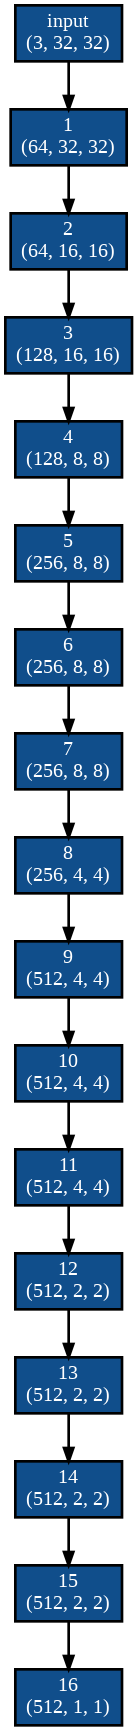
\includegraphics[clip,scale=0.25]{base.png}
      \caption{グラフ(c)}
      \label{fig:base}
    \end{minipage}
    %---- 図はここまで ----------------------
  \end{tabular}
\end{figure*}

図~ の四角が各ブロックの出力を示し, 太線がVGGのレイヤー, 点線がショートカットを表している.

\section{今後の予定}
% なんとなくなんかの勉強をするとかではなく具体的に

\begin{itemize}
  \item ショートカット関数の改善
  \item $\beta$周りの改良
\end{itemize}

\section{ソースコード}
% 埋め込みでもGitでもいいので参照できるように
githubのnotebookリポジトリ参照

% 参考文献リスト
\bibliographystyle{unsrt}
\bibliography{ref}
\end{document}
